\documentclass{article}

\usepackage{dirtree}

\usepackage[
  height=9in,      % height of the text block
  width=7.5in,       % width of the text block
  top=78pt,        % distance of the text block from the top of the page
  headheight=48pt, % height for the header block
  headsep=12pt,    % distance from the header block to the text block
  heightrounded,   % ensure an integer number of lines
        % show the main blocks
  verbose,         % show the values of the parameters in the log file
]{geometry}
\setlength{\parindent}{0pt}
\usepackage{amsmath}
\usepackage{courier}
\usepackage{graphicx}
\usepackage{amsmath}
\usepackage{booktabs}
\usepackage{fancyhdr}
\usepackage{float}
\usepackage{mathtools}

\pagestyle{fancy}
\fancyhead[L]{Pattern and Speech Recognition WS1617\\ Assignment 07}
\fancyhead[R]{ Vinh Thinh Ho (2562630) \\ Noshaba Cheema (2562653)}

\renewcommand{\headrulewidth}{0.35pt}
\newcommand\tab[1][1cm]{\hspace*{#1}}

\begin{document}
\section*{Exercise 7.1}
a)\\
b) See \textbf{multilayer\_perceptron.py}:\\
Accuracy:
\begin{itemize}
\item (i) Gradient Descent: 0.8865
\item (ii) Gradient Descent with Momentum with momentum parameter = 0.5: 0.9015
\item (iii) AdaGrad with initial accumulator value = 0.1: 0.6659
\item (iv) RMSProp with decay = 0.9, momentum = 0: 0.9321
\end{itemize}
c)\\
Update rule of Gradient Descent:
\begin{align*}
\theta = \theta - \epsilon_{k}.G
\end{align*}
Update rule of AdaGrad:
\begin{align*}
r &= r + G^TG\\
\theta &= \theta - \frac{\epsilon}{\sqrt{r}}.G
\end{align*}

In AdaGrad optimizer, with gradient G having large magnitude, we have accumulation variable $r$ also large. Observe that the pure learning rate $\epsilon$ is already small like in Gradient Descent, this will lead to the situation that we update the parameter $\theta$ with gradient G scaled by an amount of $\frac{\epsilon}{\sqrt{r}}$, which is very small. Hence, we would need more training epochs with AdaGrad in comparison with Gradient Descent to reach the local minimum. However, both 2 optimizers are tested with the same number of epochs (5 epochs), it is clear that Gradient Descent performs better then AdaGrad.
\section*{Exercise 7.2}
a) See \textbf{7.2ab.py}:\\
b) See \textbf{7.2ab.py}:\\
c)
\begin{figure}[ht]
	\centering
	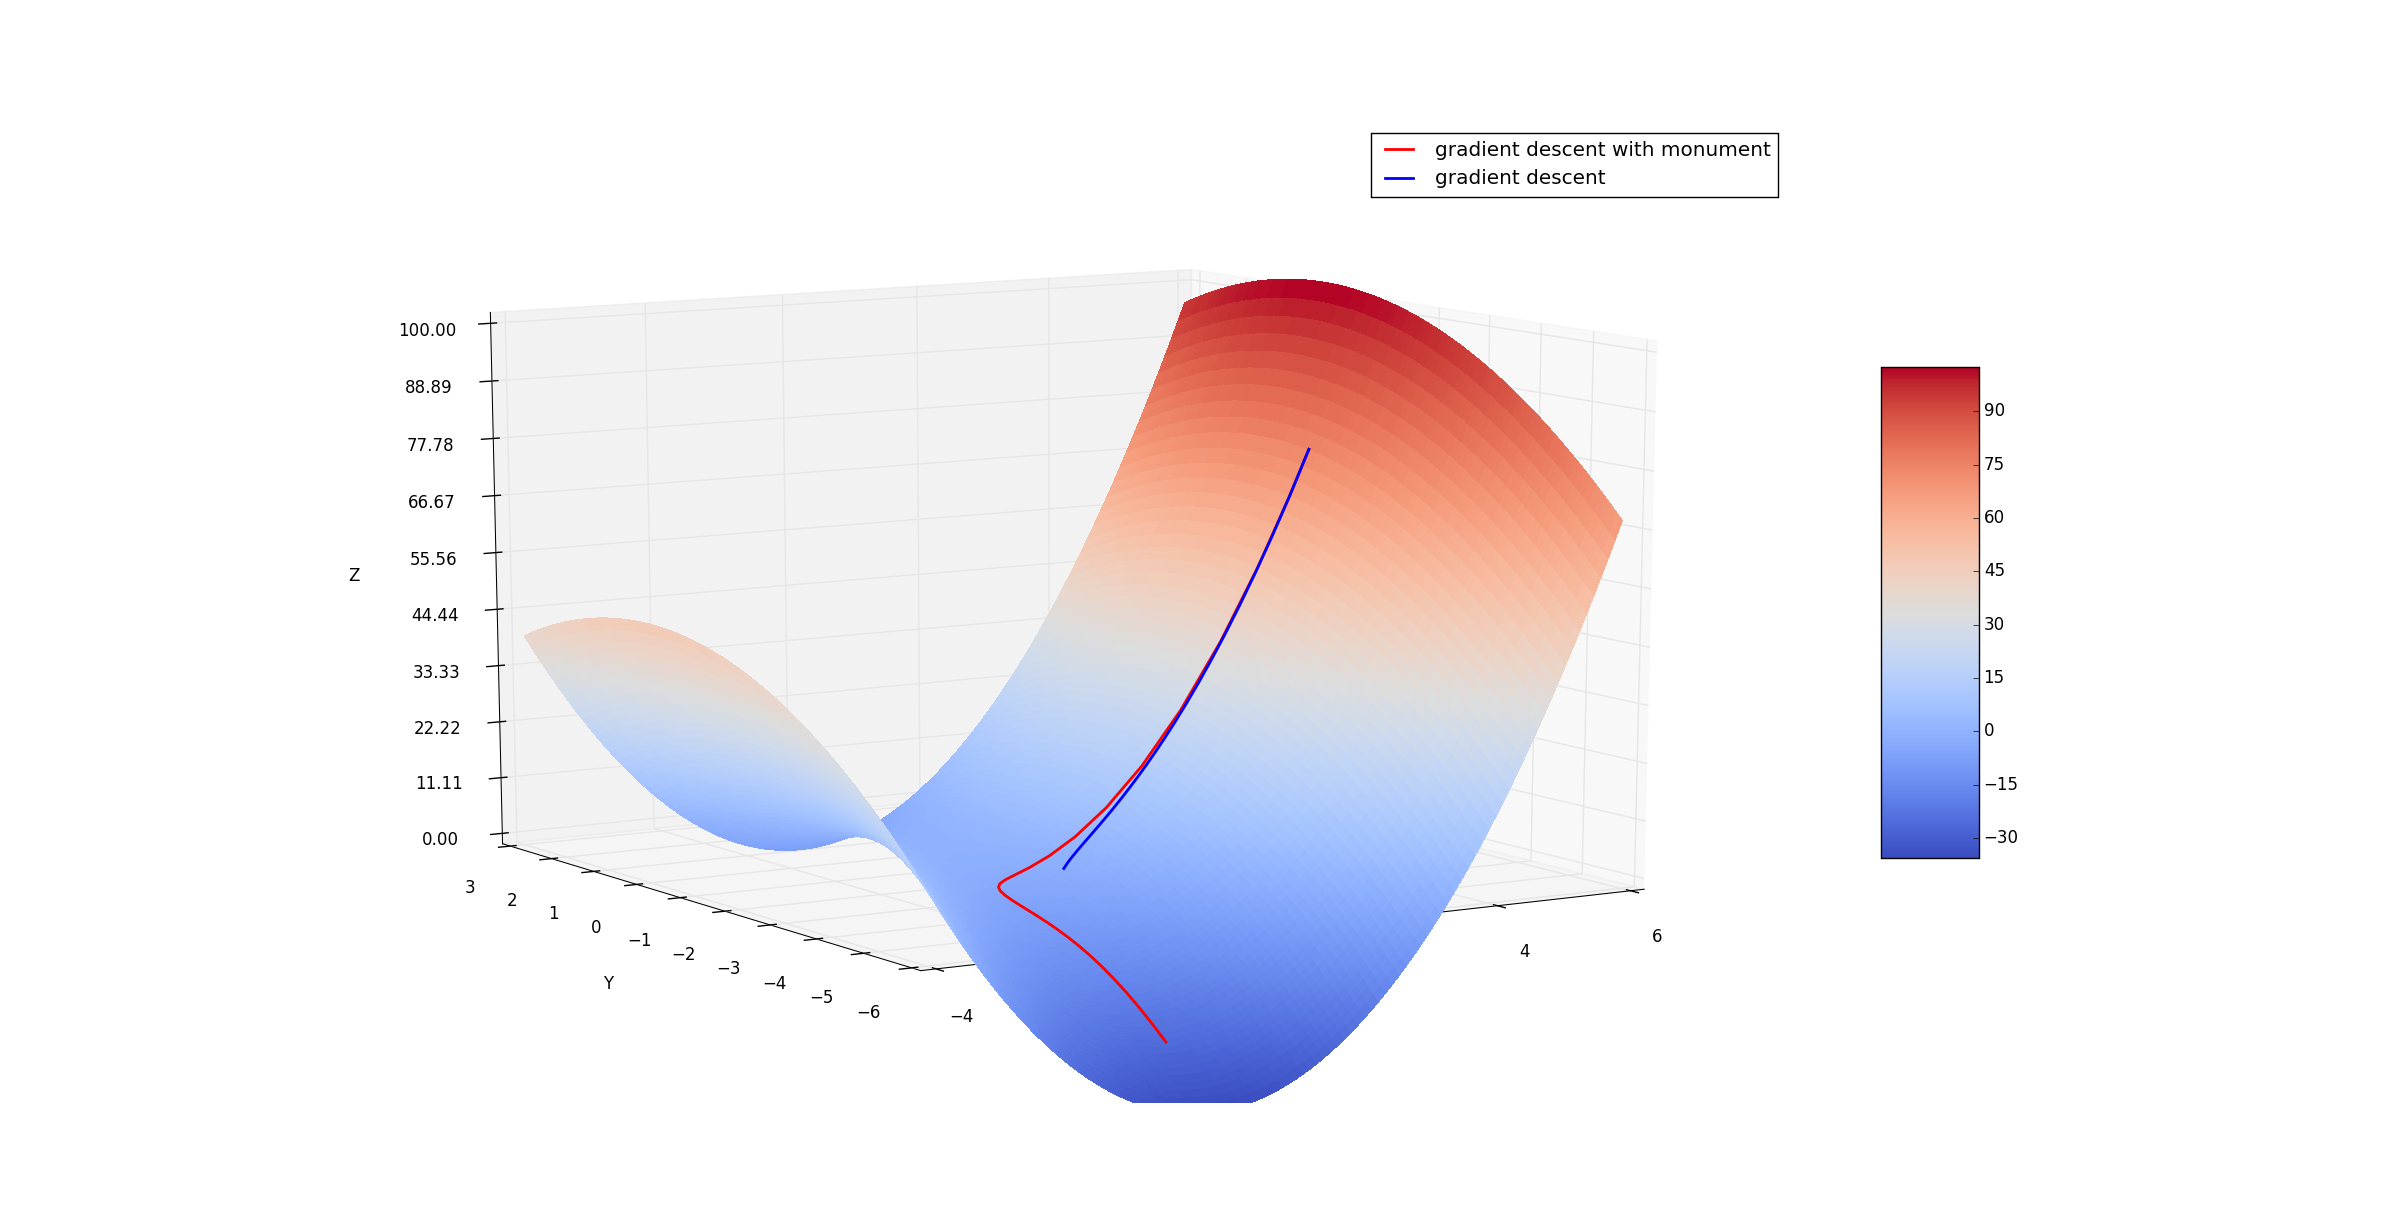
\includegraphics[scale=0.25]{72.png}
\end{figure}
\newpage
d)\\
After 30 iterations:\\
\begin{itemize}
\item GD stops at point: (0.781278030833, -1.811361584103) with loss = -1.449844703977
\item GD with Monument stops at point: (0.017928494126, -5.035721987536) with loss = -25.357531643053
\end{itemize}

Hence, we can see that Gradient Descent with Monument works better than Normal Gradient Descent in minimizing this function $3x^2 - y^2$.\\\\
e) See \textbf{7.2e.py}

\begin{figure}[ht]
	\centering
	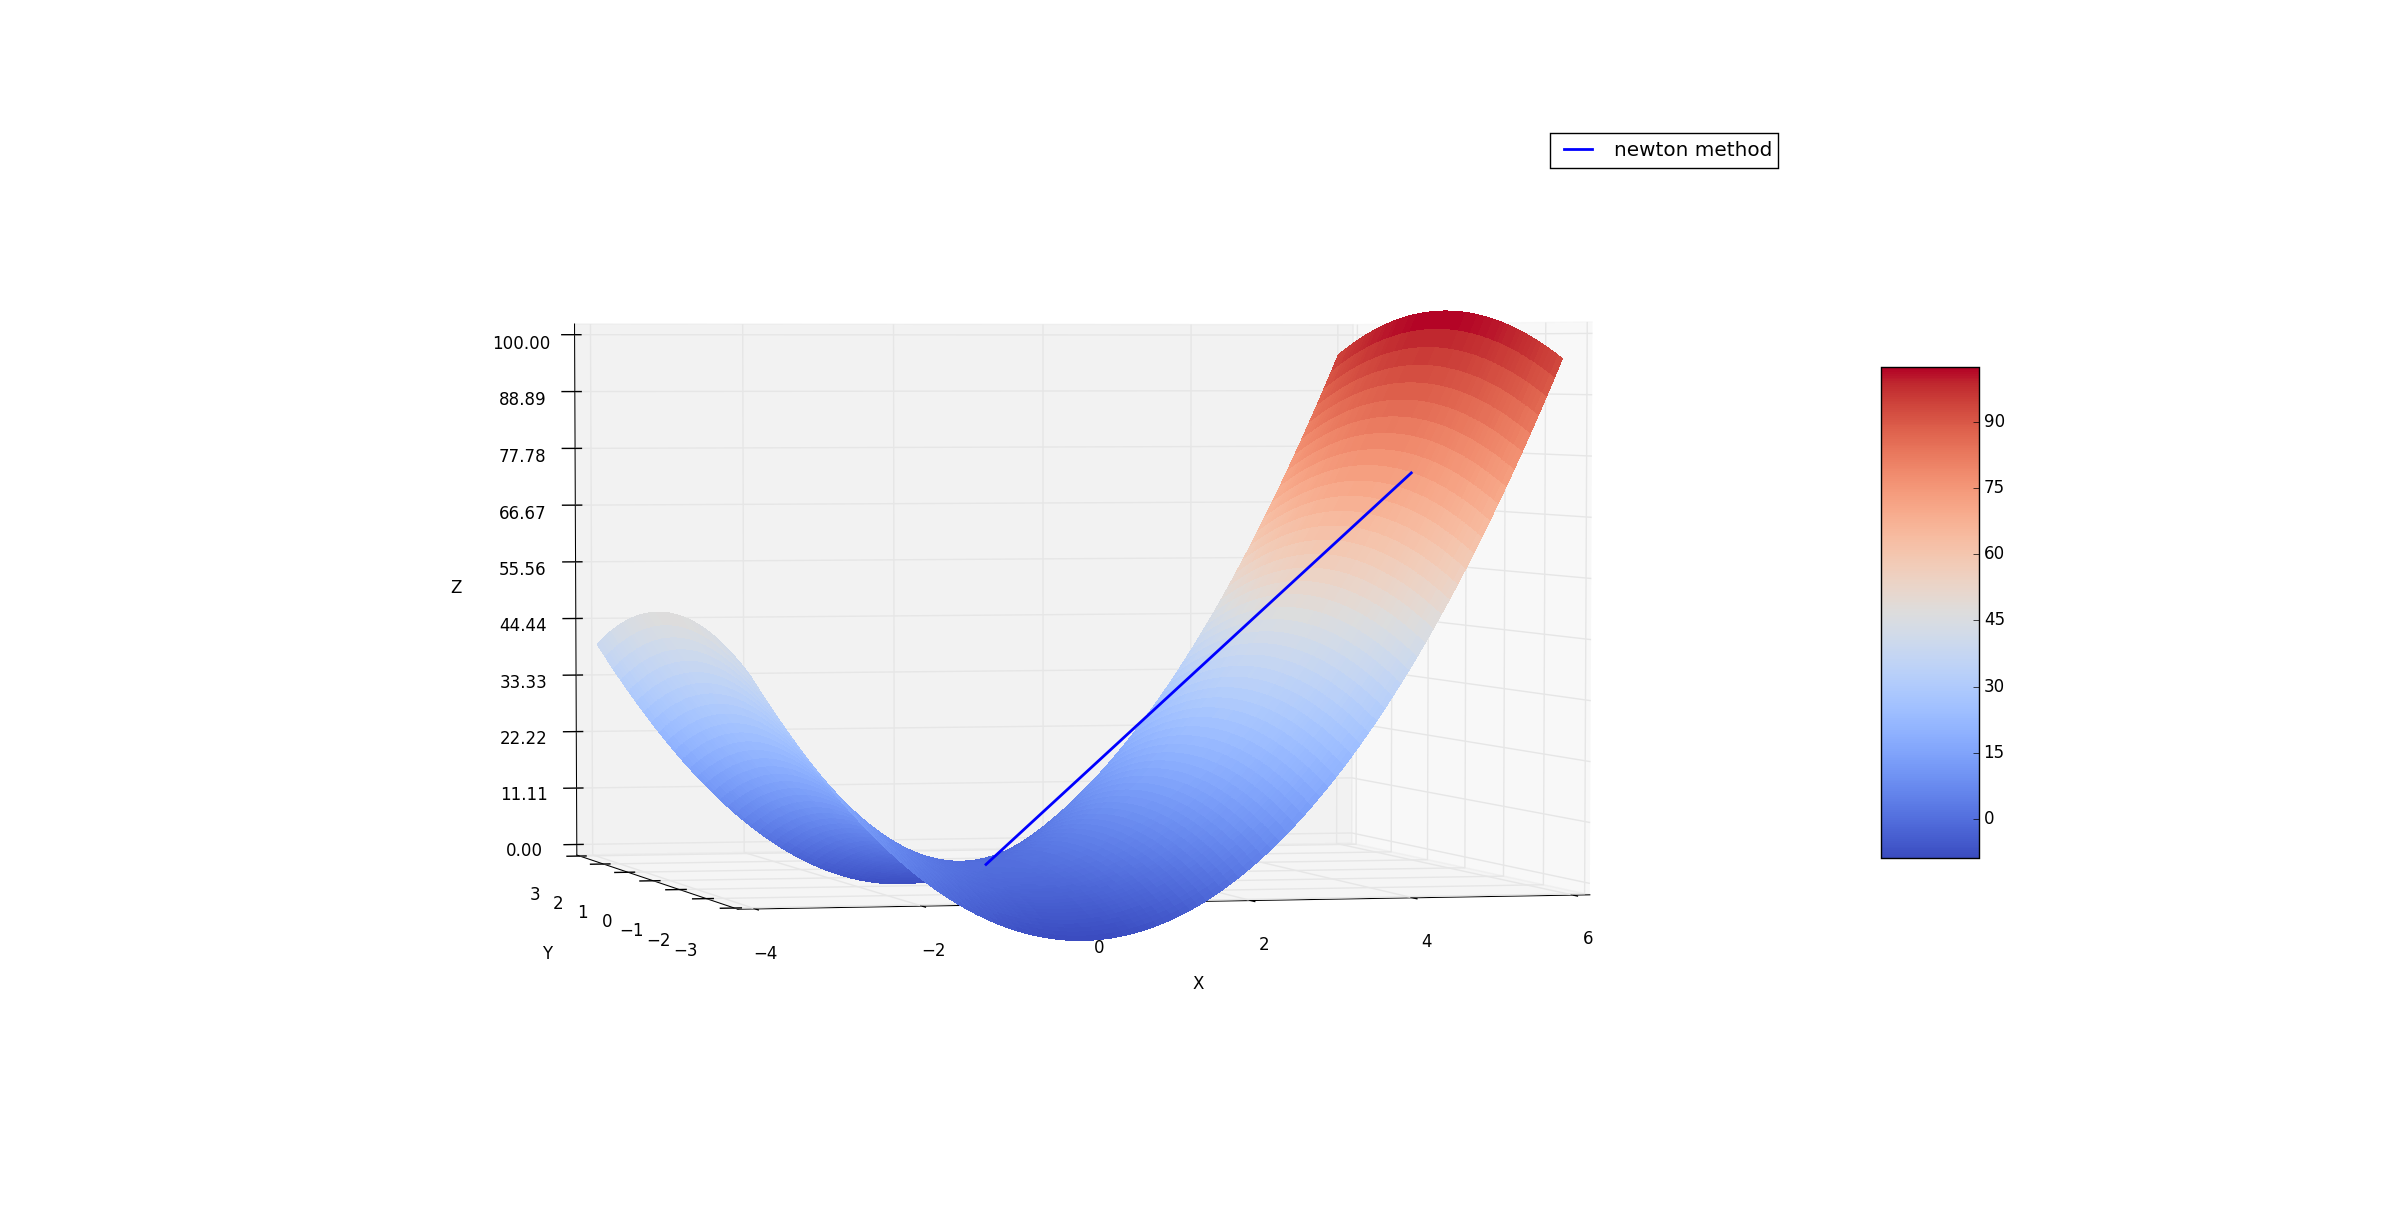
\includegraphics[scale=0.3]{72e.png}
\end{figure}

Analyzing the steps of Newton method we have:
\begin{itemize}
\item Step 1: old\_(x,y) = (5, -1); Gradient = (5, -1); new\_(x,y) = (0, 0); loss = 0
\item Step 2: old\_(x,y) = (0, 0); Gradient = (0, 0); new\_(x,y) = (0, 0); loss = 0
\item Step 3: old\_(x,y) = (0, 0); Gradient = (0, 0); new\_(x,y) = (0, 0); loss = 0
\item Step 4: old\_(x,y) = (0, 0); Gradient = (0, 0); new\_(x,y) = (0, 0); loss = 0
\item Step 5: old\_(x,y) = (0, 0); Gradient = (0, 0); new\_(x,y) = (0, 0); loss = 0);
\end{itemize}

After the first step, the method will jump to the saddle point (0, 0) which has gradient zero. The next steps from 2 to 5 will stay at this saddle point. This is an example showing why plain vanilla Newton method is not suited for training deep neural networks. The reason is in deep neural network, the loss function is typically non-convex (has a lot of extreme points), hence, when we need to minimize the loss function, we actually need some methods that could help us get away from these local maximum or saddle points. Meanwhile, Newton method always looks at points with zero gradient (could be local minimum, local maximum or saddle point), so it is not suitable for our purpose.
\newpage
\section*{Exercise 7.3}
a) See \textbf{7.3.py}\\
b) See \textbf{7.3.py}\\
c)
\begin{figure}[ht]
	\centering
	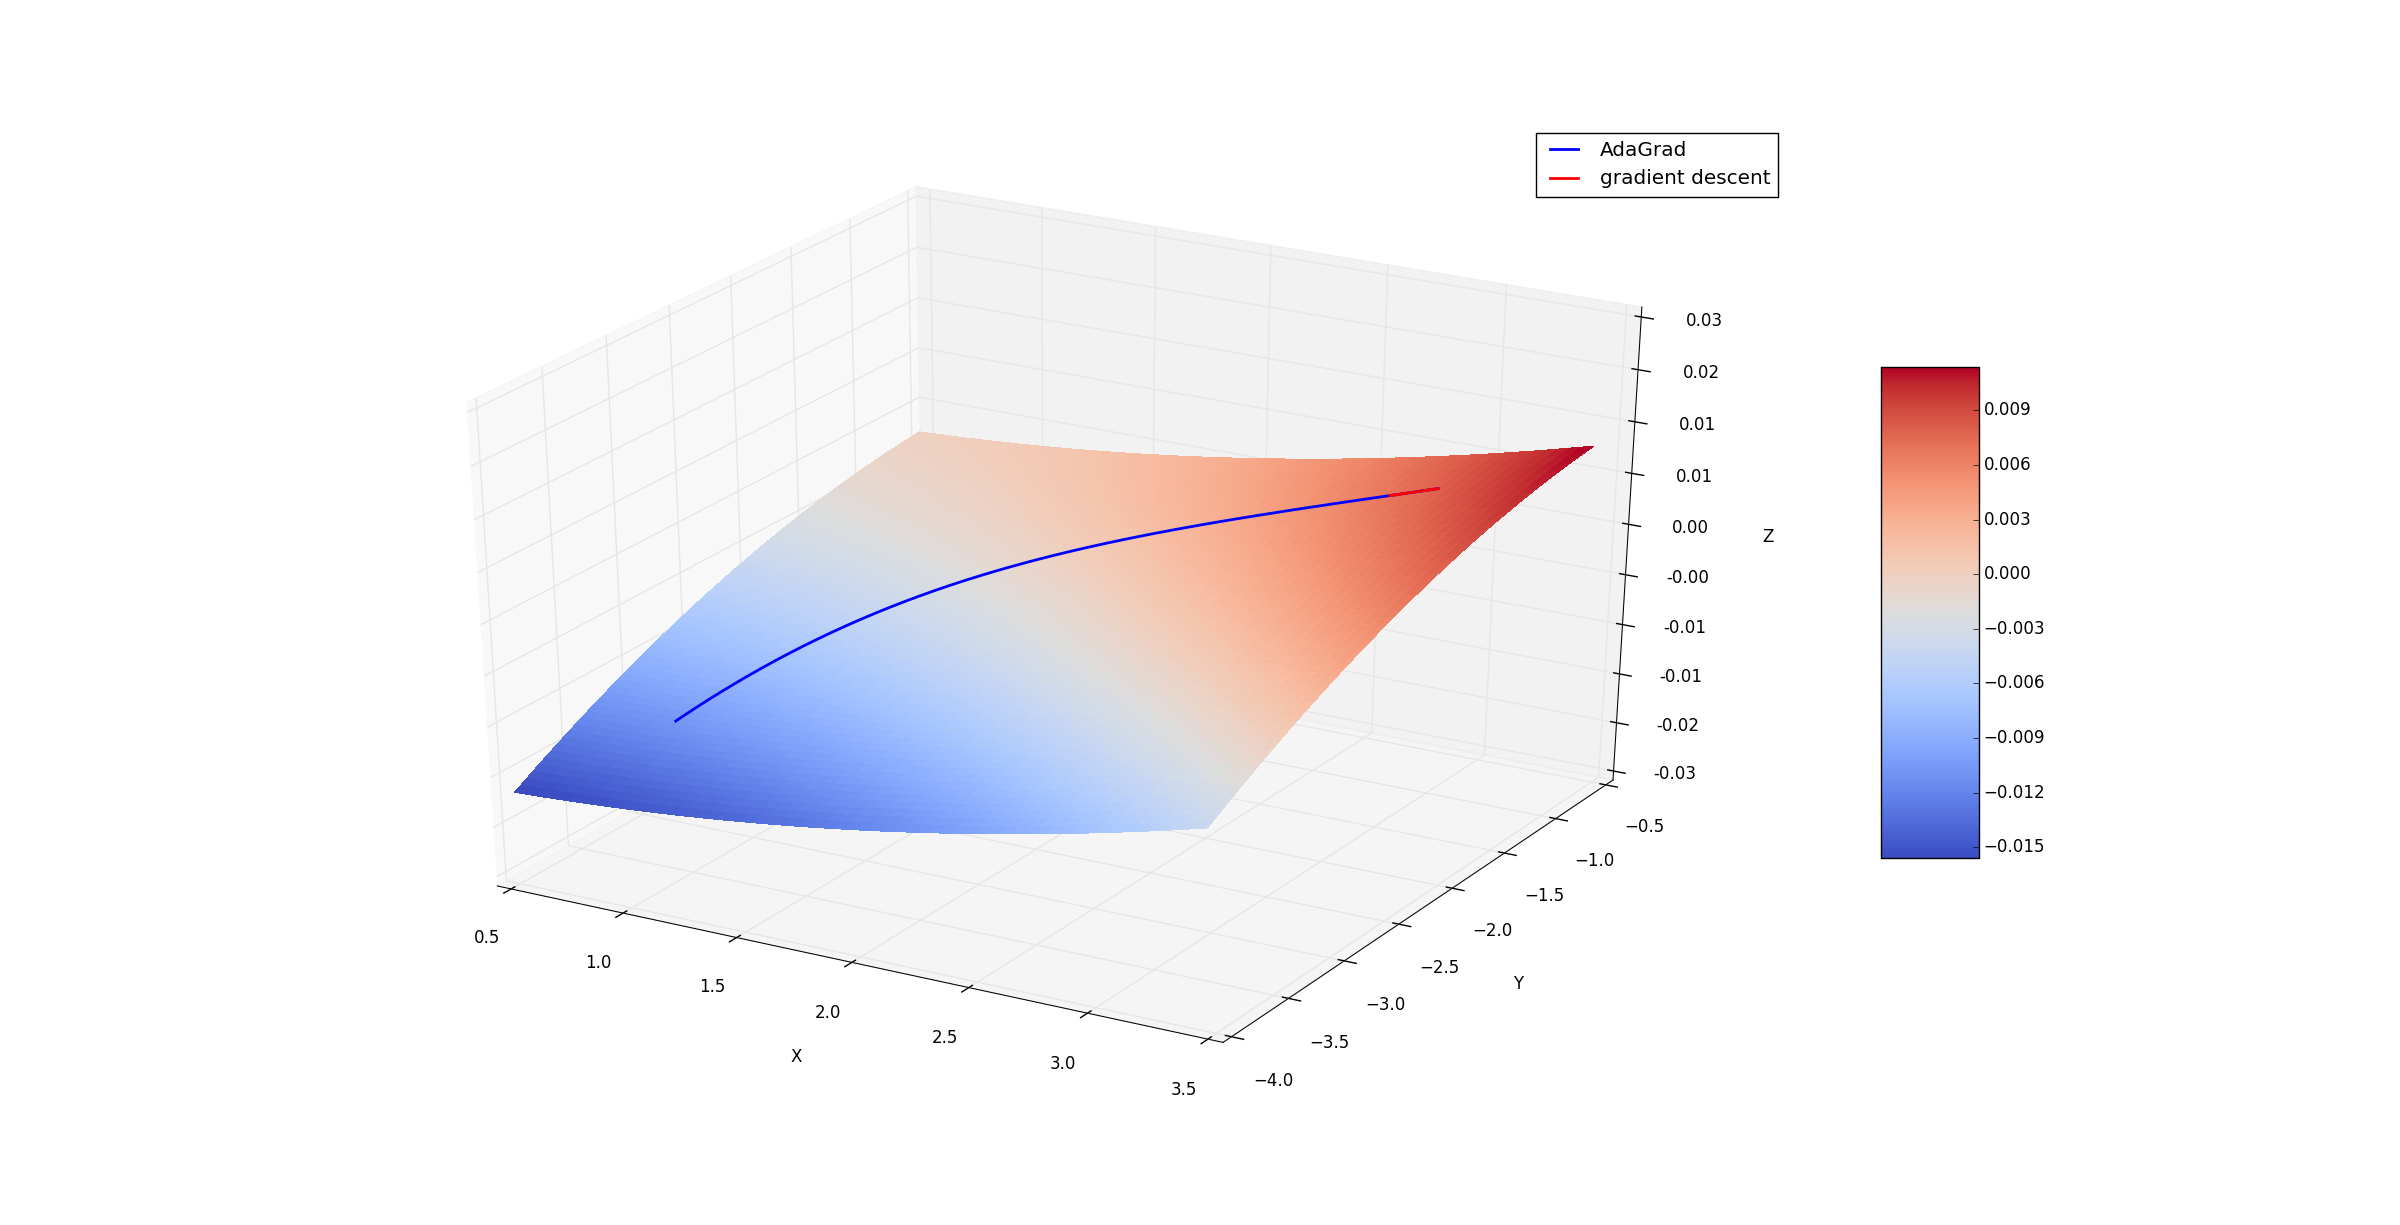
\includegraphics[scale=0.3]{73.png}
\end{figure}

\end{document}



